\documentclass[a4paper,12pt]{article}

\usepackage[utf8]{inputenc}
\usepackage[T1]{fontenc}
\usepackage[english]{babel}
\usepackage{listings}
\usepackage[breaklinks]{hyperref}
\usepackage{graphicx} % per inserir imatges
\usepackage{amsmath, amssymb} % per fórmules
\usepackage{hyperref} % enllaços
\usepackage{csquotes} % cometes tipogràfiques
\usepackage{lscape}
\usepackage{booktabs}
\usepackage{float}
\usepackage{adjustbox}
\usepackage[style=apa,backend=biber]{biblatex}
\addbibresource{referencesforrepli.bib}

\lstset{
	language=R,
	breaklines=true,
	basicstyle=\ttfamily\small
}

\begin{document}

	\title{Replication Paper (POP77082 -- Assignment) \\ 
	\begin{large} 
	The past, Brexit, and the future in Northern Ireland: a quasi-experiment (by Amélie Godefroidt, Karin Dyrstad \& Kristin Bakke)
	\end{large} }
	\author{Rubèn Llorens Poblador}
	\date{1 April 2026}
	
	\maketitle
	
	\section{Original Study}

	I will replicate the study \textit{Amélie Godefroidt, Karin Dyrstad \& Kristin Bakke (2023) The past, Brexit,
	and the future in Northern Ireland: a quasi-experiment, Journal of Elections, Public Opinion
	and Parties, 33:1, 149-161}.\\
	
	In this quasi-experiment, \textcite{godefroidt2023past} examine the effect of the Brexit referendum outcome on citizens’ perceptions in Northern Ireland regarding the causes of the conflict period known as \textit{the Troubles}, as well as on their preferences concerning the region’s future constitutional status. The rationale for the study is captured in the following passage: “Both the Brexit campaign and the referendum outcome may have prompted the Northern Irish to reminisce about the dark days of ‘the Troubles’, to worry about political and economic instability, and to feel neglected by Westminster. All of this, we argue, may have shaped their attitudes towards the key cleavages of the conflict and their preferences for Northern Ireland’s political future” \parencite[p. 151]{godefroidt2023past}.\\
	
	In their quasi-experimental design, the authors treat the outcome of the Brexit referendum as an exogenous shock. With regard to data, they benefit from the fact that the vote took place during the fieldwork of the \textit{Post-conflict Attitudes for Peace} (PAP) survey. The PAP survey was conducted between 10 May and 16 July 2016, while the referendum took place on 23 June of the same year.

	\section{Data}
		
	Although the replication materials should now be available on Harvard Dataverse, I initially obtained them directly from Professor Amélie Godefroid, as they were not accessible through the repository at the time.\\
	
	\begin{lstlisting}[language=R]
# Load and subset data
#~~~~~~~~~~~~~~~~~~~~~~~~~~~~~~~~~~~~~~~~~
Brexit <- read_dta("C:/Users/Usuario/Documents/GitHub/StatsII_2026/replication/my_replication_paper_RLP/GodefroidtDyrstadBakke_2022_ReplicationFiles/Data/Brexit.dta")


\end{lstlisting}

	\section{Original Models}
	
	First, the authors created a control group (respondents surveyed before the Brexit referendum) and a treatment group (those surveyed after the referendum outcome was known). This variable, however, is already included in the replication dataset under the name \texttt{referendum}.\\
	
	\textcite{godefroidt2023past} present five figures in their original article. I replicate them in sequence and provide a simplified version of the code required to produce each of them.\\
	
	Figure 1 displays the change in the perceived importance (measured as differences in means) attributed to specific causes of the Troubles following the referendum. It highlights a significant increase in the perceived relevance of Westminster rule and the partition of Ireland.


	\begin{lstlisting}[language=R]
	# 1. Extracting coefficients and Confidence Intervals (example for one group)
	cis.rc.em <- matrix(NA, length(rootcauses), 2)
	b.rc.em <- matrix(NA, length(rootcauses), 1)
	
	for (i in 1:length(rootcauses)) {
		b.rc.em[i] <- ate.rc.em[[i]]$coefficients[2]
		ci <- confint(ate.rc.em[[i]])
		cis.rc.em[i,] <- cbind(ci[2,1], ci[2,2]) # Lower and Upper bounds
	}
	
	# 2. Graphics environment setup
	# mfrow=c(1,2) creates the side-by-side panels for Figure 1
	par(mfrow=c(1,2), mar = c(5, 4, 0, 2), oma = c(0.5, 3.5, 0, 0))
	
	# 3. Constructing the first panel (Root Causes)
	plot(b.rc.c, y.lab, type="n", xlim = c(-0.5, 0.5), ylim = c(0.5, 4.5), 
	yaxt="n", xlab = "Difference in Means")
	axis(2, at=y.lab, labels=rc.vnames, las = 2, cex.axis=0.9)
	
	# Data layers: Matching (circles), Controls (crosses), and No Correction (triangles)
	points(b.rc.em, y.lab, pch=21, col = "black") # Entropy Matching
	segments(cis.rc.em[,1], y.lab, cis.rc.em[,2], y.lab, lwd=1.5)
	
	# Applying 'jitter' to prevent overlapping symbols
	points(b.rc.c, y.lab + jitter.c, pch=4, col = "grey20") # Covariates
	segments(cis.rc.c[,1], y.lab + jitter.c, cis.rc.c[,2], y.lab + jitter.c, lty=2)
	
	abline(v=0, lty=1) # Reference line at zero (Null Hypothesis)
	
	# 4. Global Legend
	# Positioned outside the plot area using par(xpd = NA) logic
	legend(x=-1.7, y=-0.4, horiz = T, bty="n",
	legend=c("Matching", "Covariates", "No Correction"),
	lty = c(1,2,4), pch=c(21,4,6))
	
	\end{lstlisting}
	
\begin{figure}[h]
	\centering
	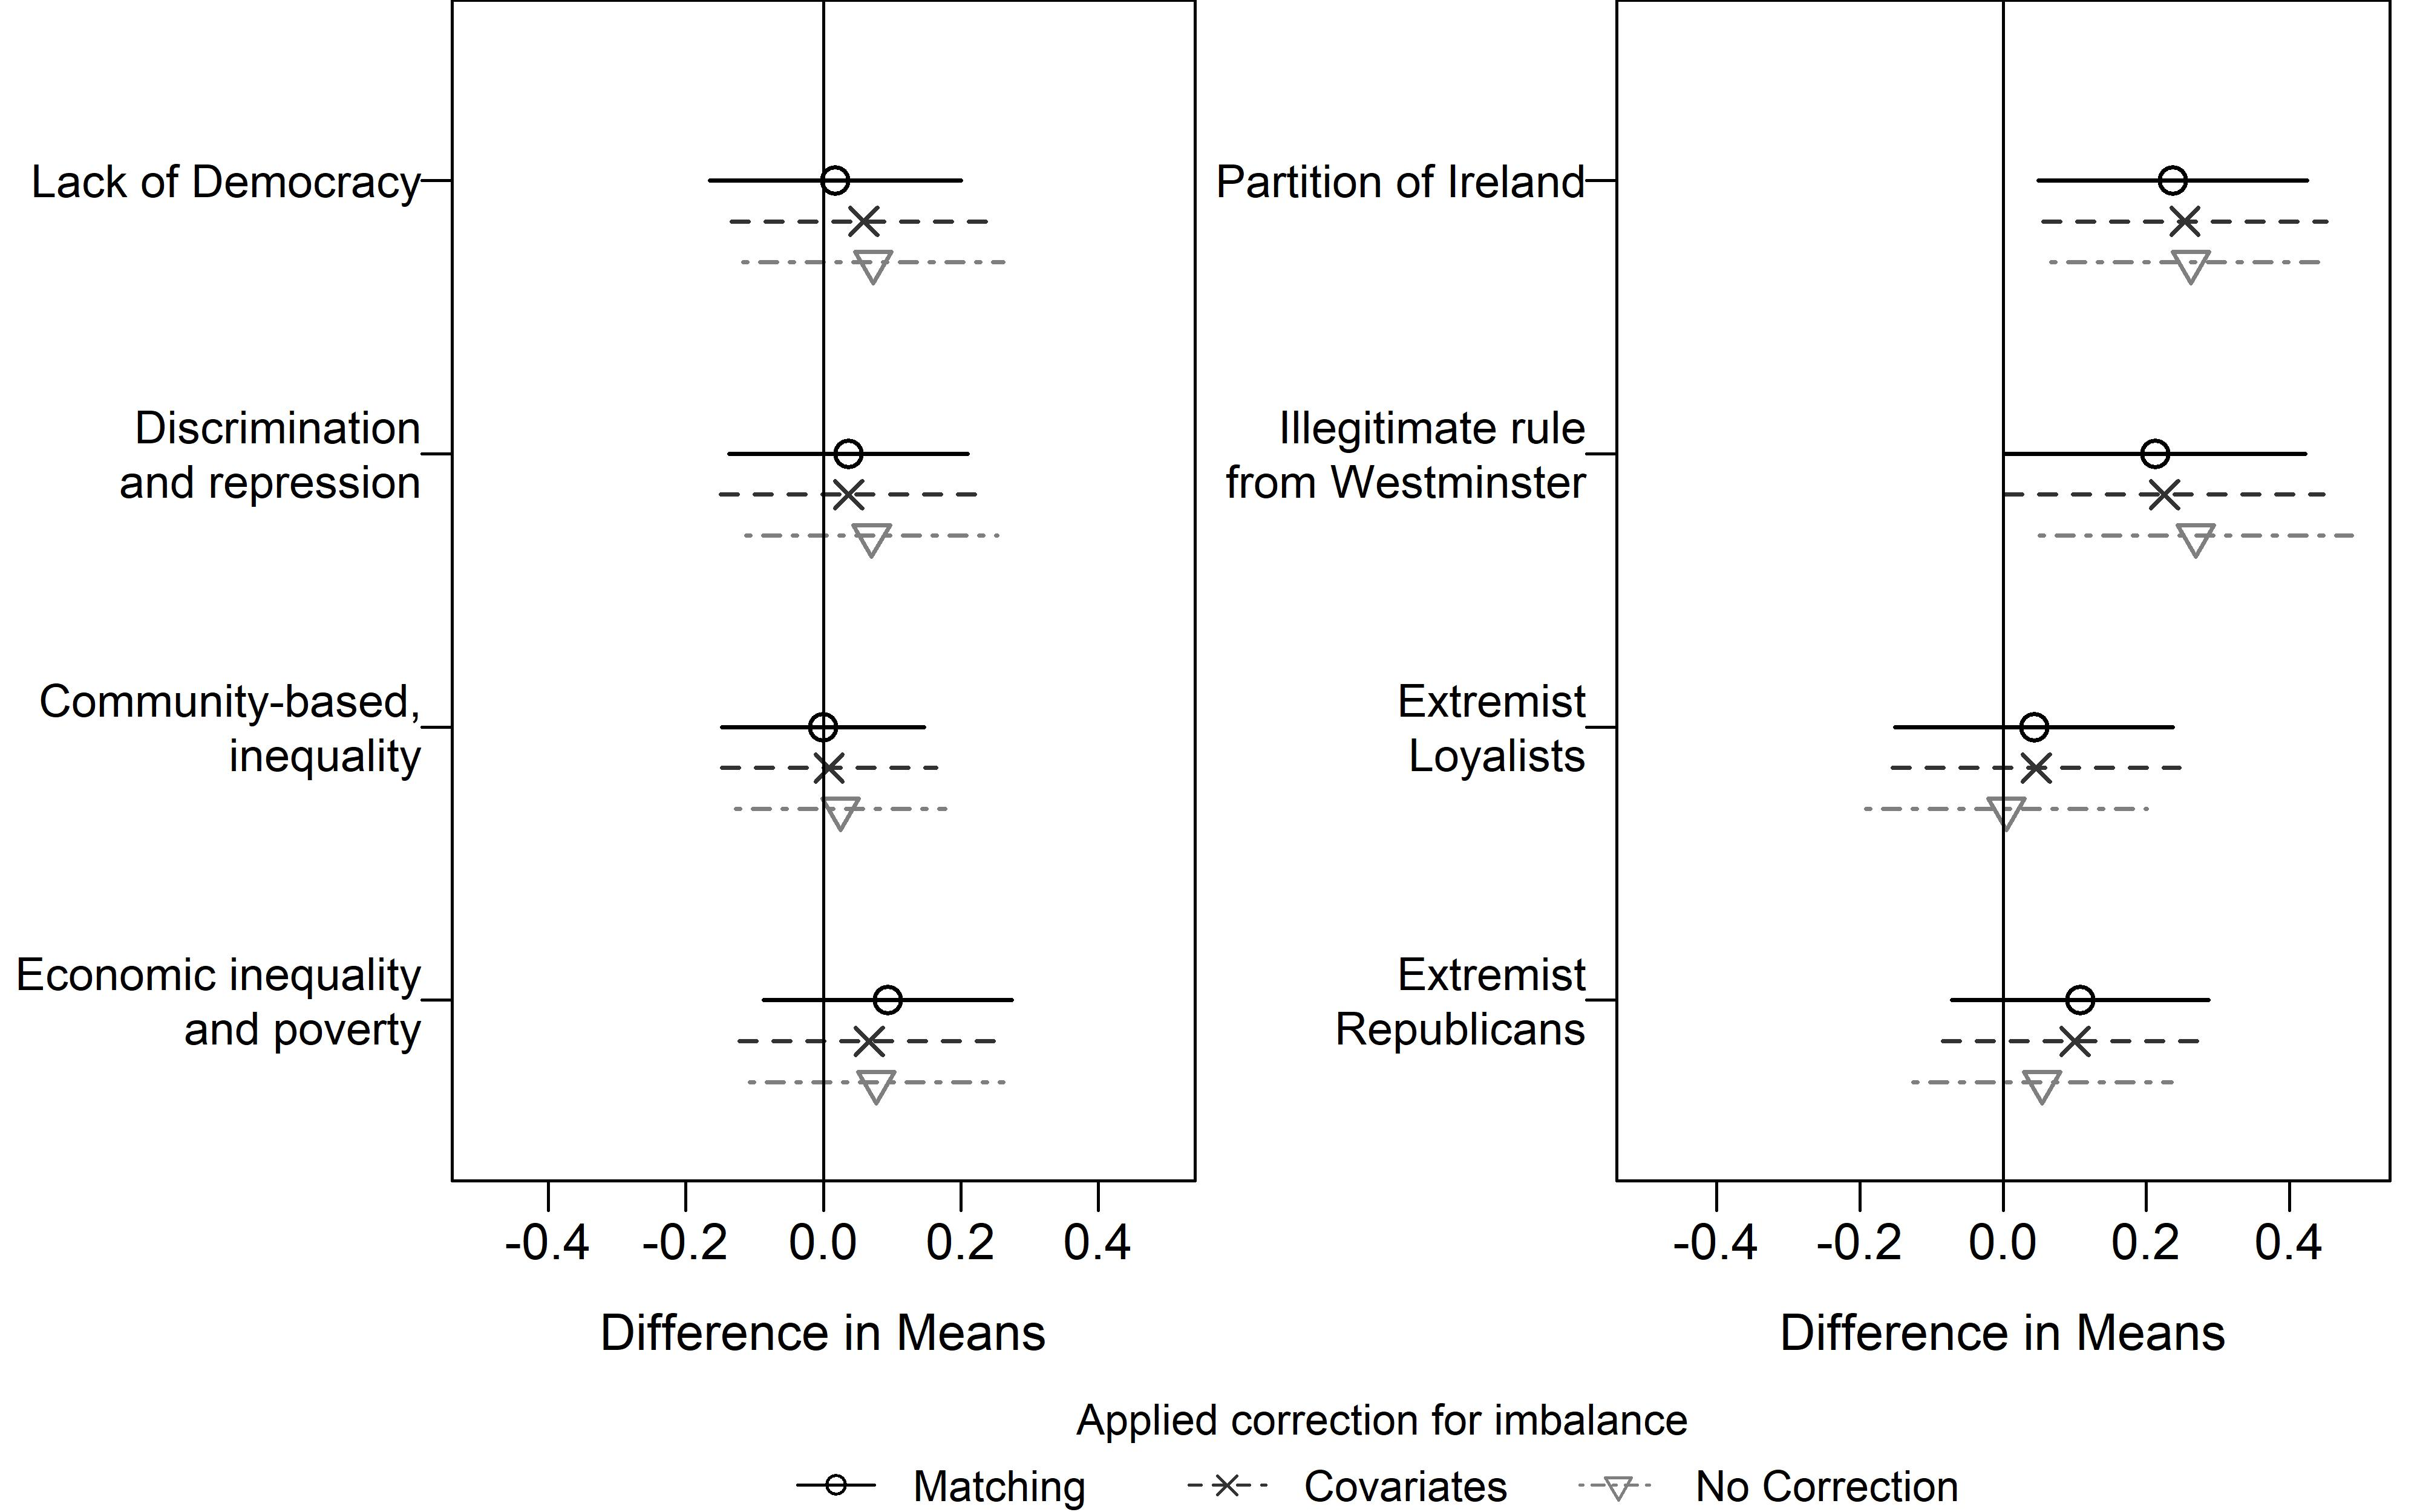
\includegraphics[width=1\textwidth]{Fig1.jpeg}
	\caption{Average treatment effect of the referendum on perceptions of conflict causes (replicated)}
	\label{fig:meva_figura_1}
\end{figure}
	
	Figure 2 shows the descriptive shift in constitutional preferences before and after the referendum outcome was known, showing a 9-percentage-point increase in support for Irish reunification and a 13-percentage-point drop in support for remaining in the UK following the Leave vote. Preferences for becoming an independent state do not appear to be affected by the treatment, as evidenced by a negligible one-percentage-point decrease.\\
	
\begin{figure}[h]
	\centering
	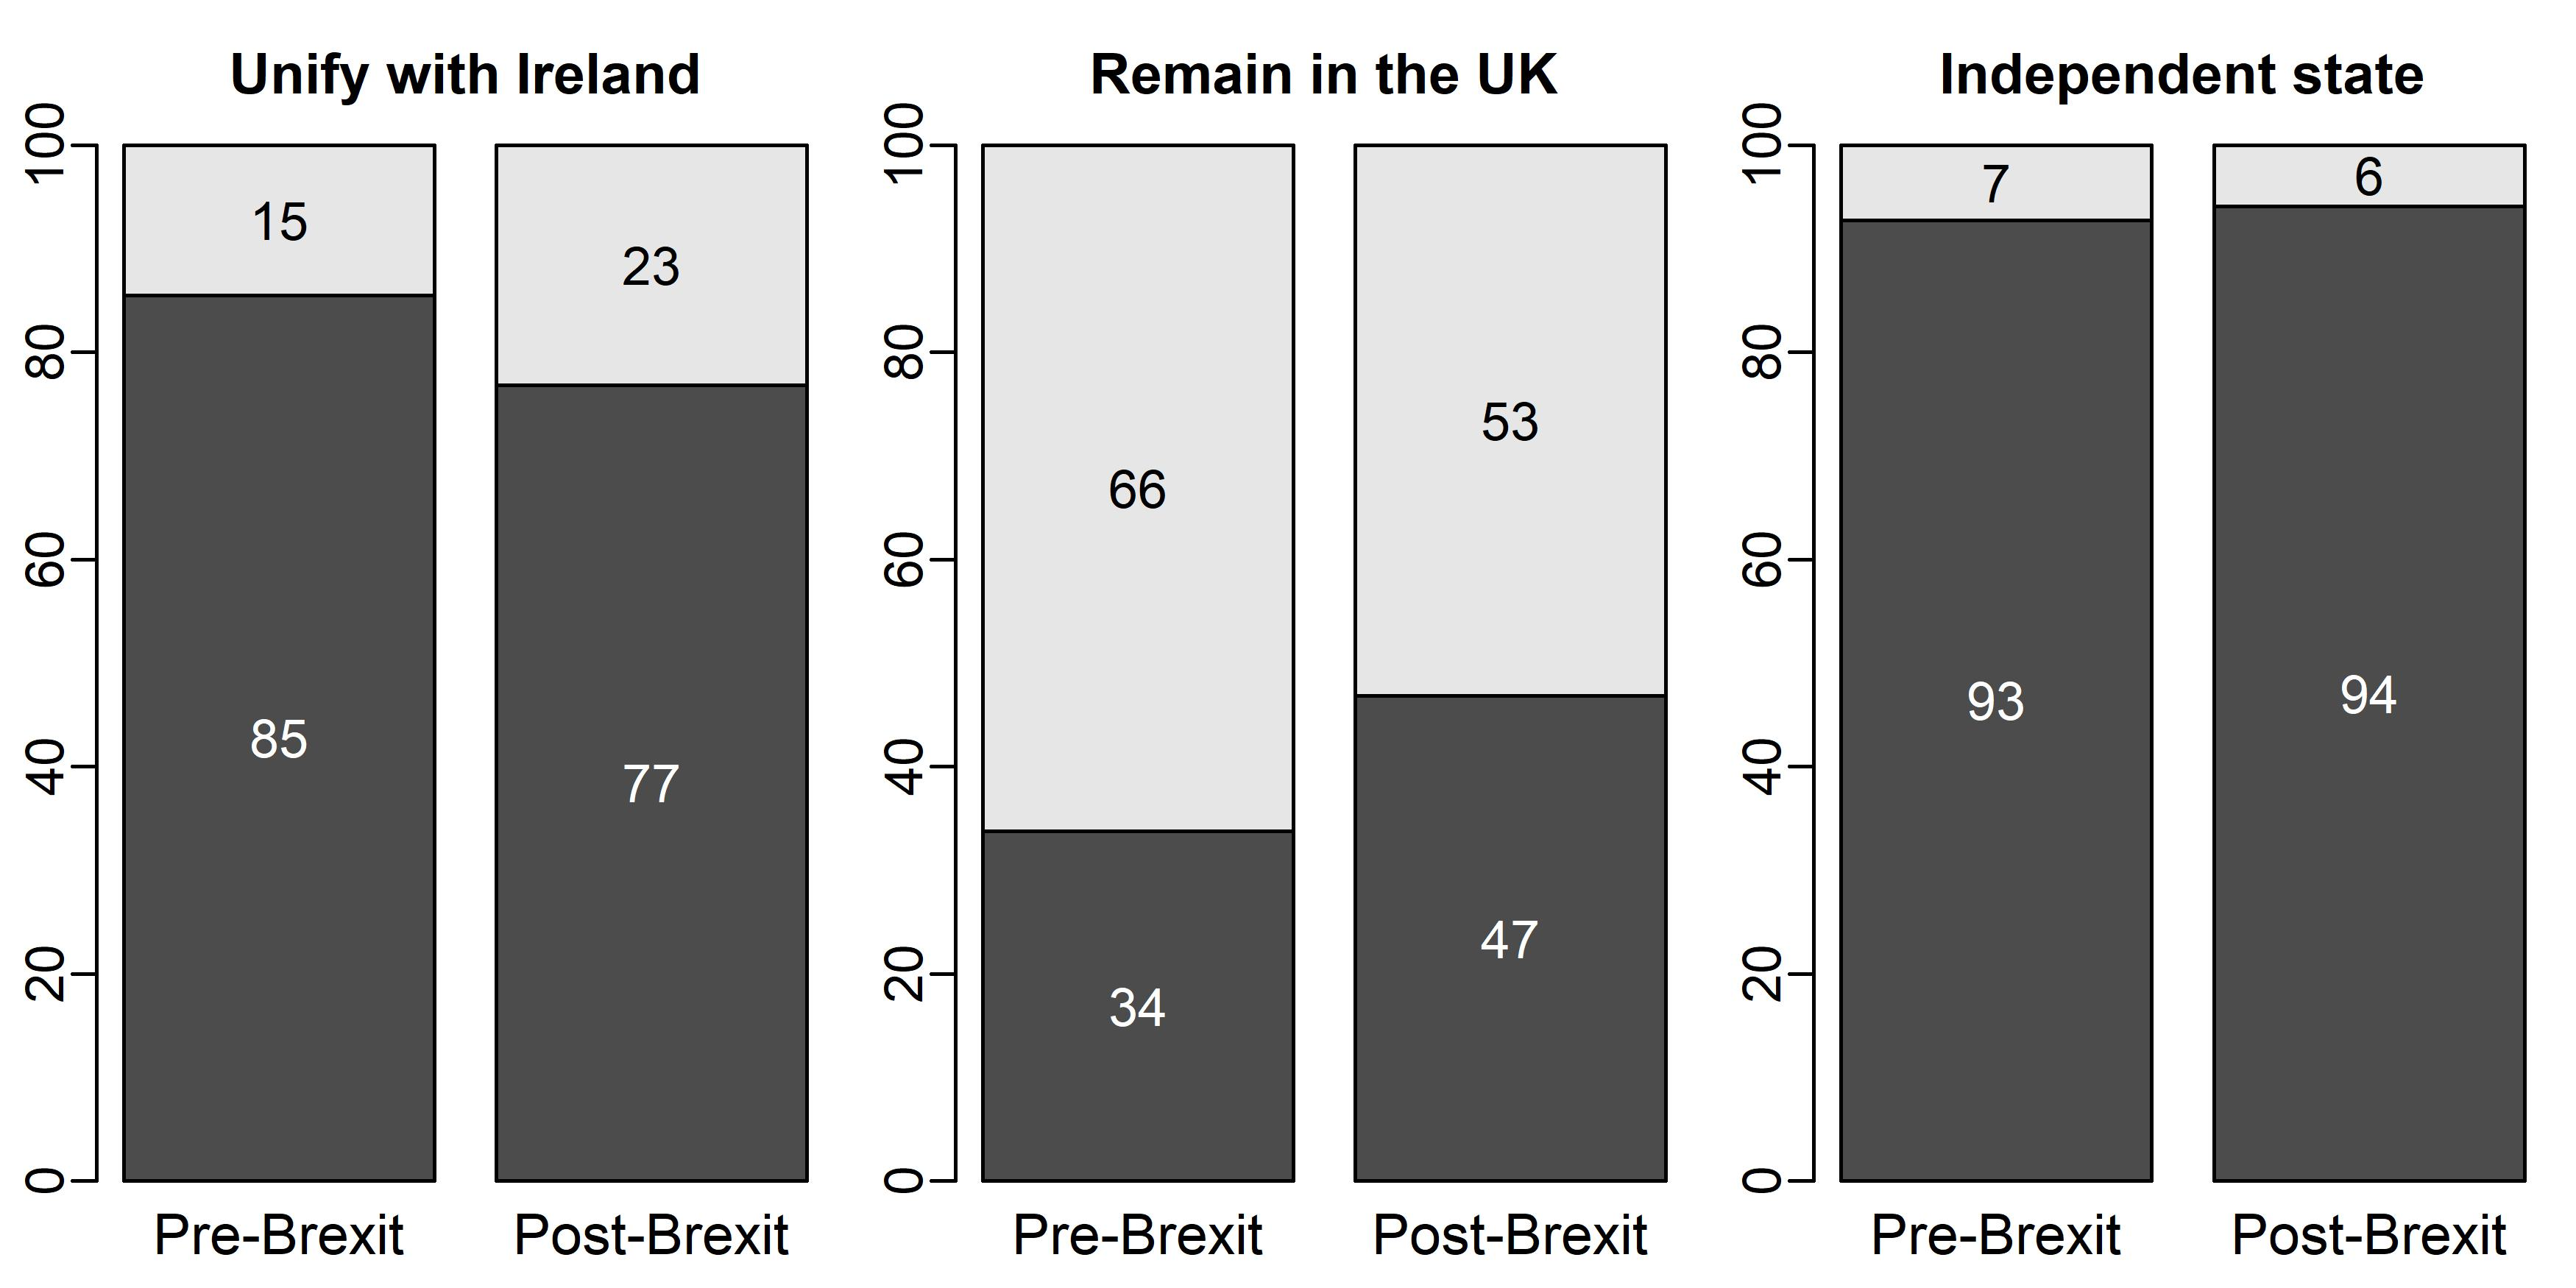
\includegraphics[width=1\textwidth]{Fig2.jpeg}
	\caption{Pre- and post-referendum preferences for the future of Northern Ireland (\%) (replicated)}
	\label{fig:meva_figura_2}
	\end{figure}

	
	\begin{lstlisting}[language=R]	
	# 1. DATA TRANSFORMATION: Create percentage tables for each preference
	# Example for 'Unification' (repeated for 'Remain' and 'Independence')
	unif_tab <- table(Brexit$unification, Brexit$referendum)
	unif_perc <- apply(unif_tab, 2, function(x){ x * 100 / sum(x, na.rm = TRUE) })
	
	# 2. PLOT SETUP: 3-panel horizontal layout
	jpeg("Fig2.jpeg", width = 7, height = 3.5, units = 'in', res = 500)
	par(mfrow = c(1, 3), mar = c(2, 2, 3, 0.5))
	
	# 3. CORE PLOTTING LOGIC (Repeated for each panel)
	# Calculate midpoints for text labels
	ys.u <- apply(unif_perc, 2, function(x) c(x[1]/2, head(cumsum(x), -1) + tail(x, -1)/2))
	xs.u <- barplot(unif_perc, names.arg = c("Pre-Brexit", "Post-Brexit"), main = "Unify with Ireland")
	
	# Add percentage labels directly onto bars
	text(rep(xs.u, each = nrow(ys.u)), c(ys.u), 
	labels = round(c(unif_perc), 0), col = c("white", "black"))
	
	# 4. STATISTICAL ESTIMATION (ATEs)
	# Define outcomes and iterate through model specifications
	future_outcomes <- Cs(remain, independence, unification)
	ate_results <- list()
	
	for (outcome in future_outcomes) {
		# Example: Model with Entropy Matching Weights
		f_formula <- as.formula(paste(outcome, "~ referendum + age + exposure")) # simplified
		ate_results[[outcome]] <- lm(f_formula, data = Brexit, weights = W.out$w)
		
		# Summary output for verification
		print(summary(ate_results[[outcome]]))
	}
	
	dev.off()
\end{lstlisting}
	
	Figure 3 provides a formal statistical test to confirm that the changes in political preferences for Northern Ireland’s future are statistically significant and robust across various model specifications.\\
	
	
	\begin{lstlisting}[language=R]		
	# 1. DATA EXTRACTION: Capture coefficients and 95% CIs for future preferences
	# Example logic for Entropy Matching (repeated for Covariates and No Correction)
	cis.f.em <- matrix(NA, length(future), 2)
	b.f.em <- matrix(NA, length(future), 1)
	
	for (i in 1:length(future)) {
		b.f.em[i] <- ate.f.em[[i]]$coefficients[2]
		ci <- confint(ate.f.em[[i]])
		cis.f.em[i,] <- cbind(ci[2,1], ci[2,2]) # Store Lower and Upper bounds
	}
	
	# 2. PLOT SETUP: Define custom labels and vertical spacing
	vnames.f <- c("Remain Part\n of the UK", "Become an\n Independent State", "Unify with the\n Rest of Ireland")
	y.lab.f <- 1:length(future)
	jitter.f.c <- -0.15; jitter.f.nc <- -0.30
	
	# 3. VISUALIZATION: Build the coefficient plot
	jpeg("Fig3.jpeg", width = 5, height = 5, units = 'in', res = 500)
	par(mar = c(5, 4, 0, 3), oma = c(0.5, 3.5, 0.5, 0.2))
	
	# Create empty plot area with custom axes
	plot(b.f.c, y.lab.f, type = "n", yaxt = "n", xlim = c(-0.5, 0.5), 
	ylim = c(0.5, 3.5), xlab = "Difference in Means", ylab = "")
	axis(2, at = y.lab.f, labels = vnames.f, las = 2, cex.axis = 0.9)
	
	# Layer 1: Entropy Matching (Black circles, solid lines)
	points(b.f.em, y.lab.f, pch = 21, lwd = 1.5)
	segments(cis.f.em[,1], y.lab.f, cis.f.em[,2], y.lab.f, lty = 1)
	
	# Layer 2: Covariate Adjustment (Grey crosses, dashed lines)
	points(b.f.c, y.lab.f + jitter.f.c, pch = 4, col = "grey20")
	segments(cis.f.c[,1], y.lab.f + jitter.f.c, cis.f.c[,2], y.lab.f + jitter.f.c, lty = 2, col = "grey20")
	
	# Reference line for null hypothesis (no effect)
	abline(v = 0, lty = 3)
	
	# 4. LEGEND: Positioned outside the plot region
	par(xpd = NA)
	legend(x = -0.75, y = -0.15, horiz = TRUE, bty = "n",
	legend = c("Matching", "Covariates", "No Correction"),
	lty = c(1, 2, 4), pch = c(21, 4, 6))
	
	dev.off()
	
\end{lstlisting}
	
\begin{figure}[h]
	\centering
	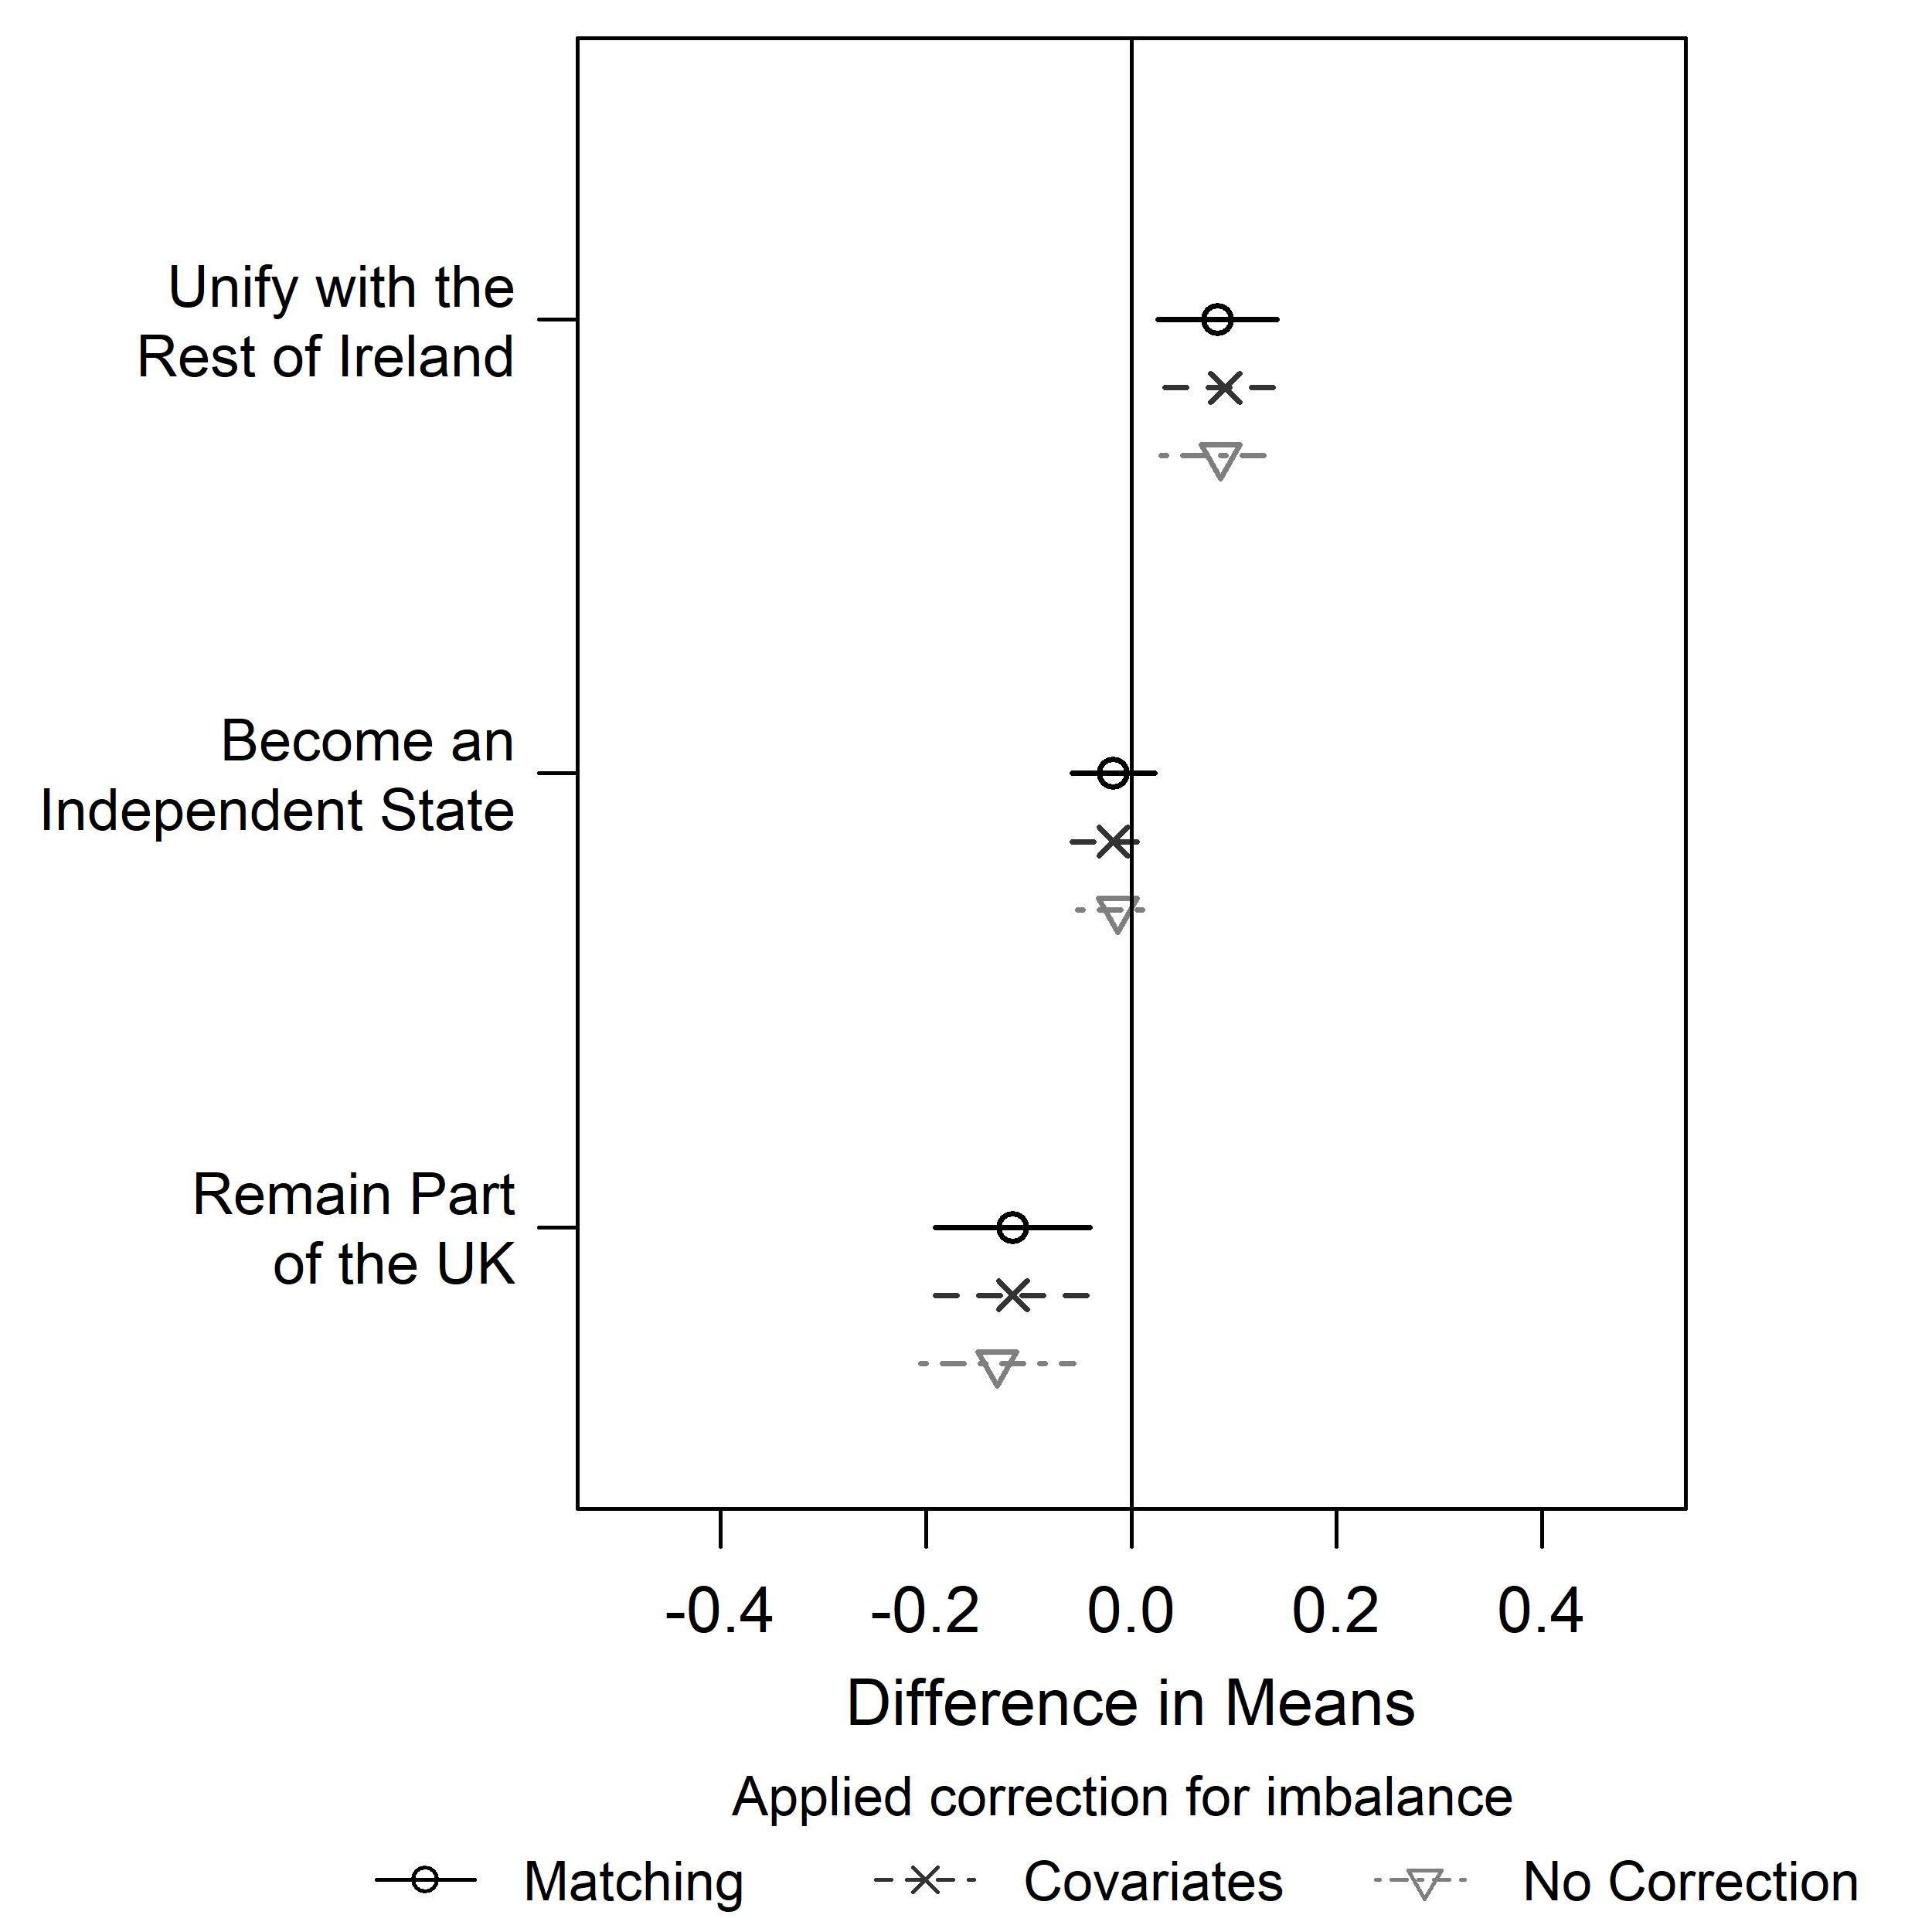
\includegraphics[width=1\textwidth]{Fig3.jpeg}
	\caption{Average treatment effect of the referendum on preferences for the future (replicated)}
	\label{fig:meva_figura_3}
\end{figure}
	
	The last two figures focus on the perceived causes of the conflict. The following code snippet illustrates how these variables are operationalised and incorporated into the empirical analysis:\\
	
	\begin{lstlisting}[language=R]	
	# Cause 1: Economic inequalities and poverty
	Brexit.1 <- Brexit %>% drop_na(cause_1, employment_1)
	W.out.1 <- weightit(referendum ~ age + employment_1 + exposure,
	data = Brexit.1, estimand = "ATT", method = "ebal") #create weights
	econ.rdd = lm(cause_1 ~ time_zero+referendum+(time_zero*referendum), data = Brexit.1,
	weights = W.out.1$w)
	Brexit.1$econ.rdd.pred <- predict(econ.rdd)
	summary(econ.rdd)
\end{lstlisting}

	Figure 4 presents a time-series view of conflict perceptions, showing that while structural causes gained importance during the campaign, blame attributed to extremist groups saw a sharp decline.\\
	
	\begin{lstlisting}[language=R]		
	# 1. GRAPHICAL LAYOUT: 4x2 Grid for the 8 distinct conflict causes
	jpeg("Fig4.jpeg", width = 7, height = 10, units = 'in', res = 500)
	par(mfrow=c(4,2), mar = c(3,3,3,2))
	
	# 2. CORE PLOTTING LOGIC (Repeated for Causes 1-8)
	# Scatter plot of raw data points (grey to de-emphasize individual variance)
	plot(Brexit.1$date, Brexit.1$cause_1, pch=1, col="grey90", 
	frame.plot = FALSE, ylim=c(0.8, 5.2), main = "Economic Inequalities")
	
	# 3. RD DISCONTINUITY LINES: Plotting predicted trends
	# Trend BEFORE referendum (referendum == 0)
	with(subset(Brexit.1, referendum==0), 
	lines(date, econ.rdd.pred, col="black", lwd=4))
	
	# Trend AFTER referendum (referendum == 1)
	with(subset(Brexit.1, referendum==1), 
	lines(date, econ.rdd.pred, col="gray", lwd=4))
	
	# 4. ANNOTATIONS: Adding the threshold and statistical results
	abline(v=as.Date("2016-06-24"), lty=2, lwd=2) # Referendum Day
	text(as.Date("2016-05-31"), 3, "0.011(0.004)\n p=.002") # Slope & Sig.
	
	dev.off()
\end{lstlisting}
	
\begin{figure}[h]
	\centering
	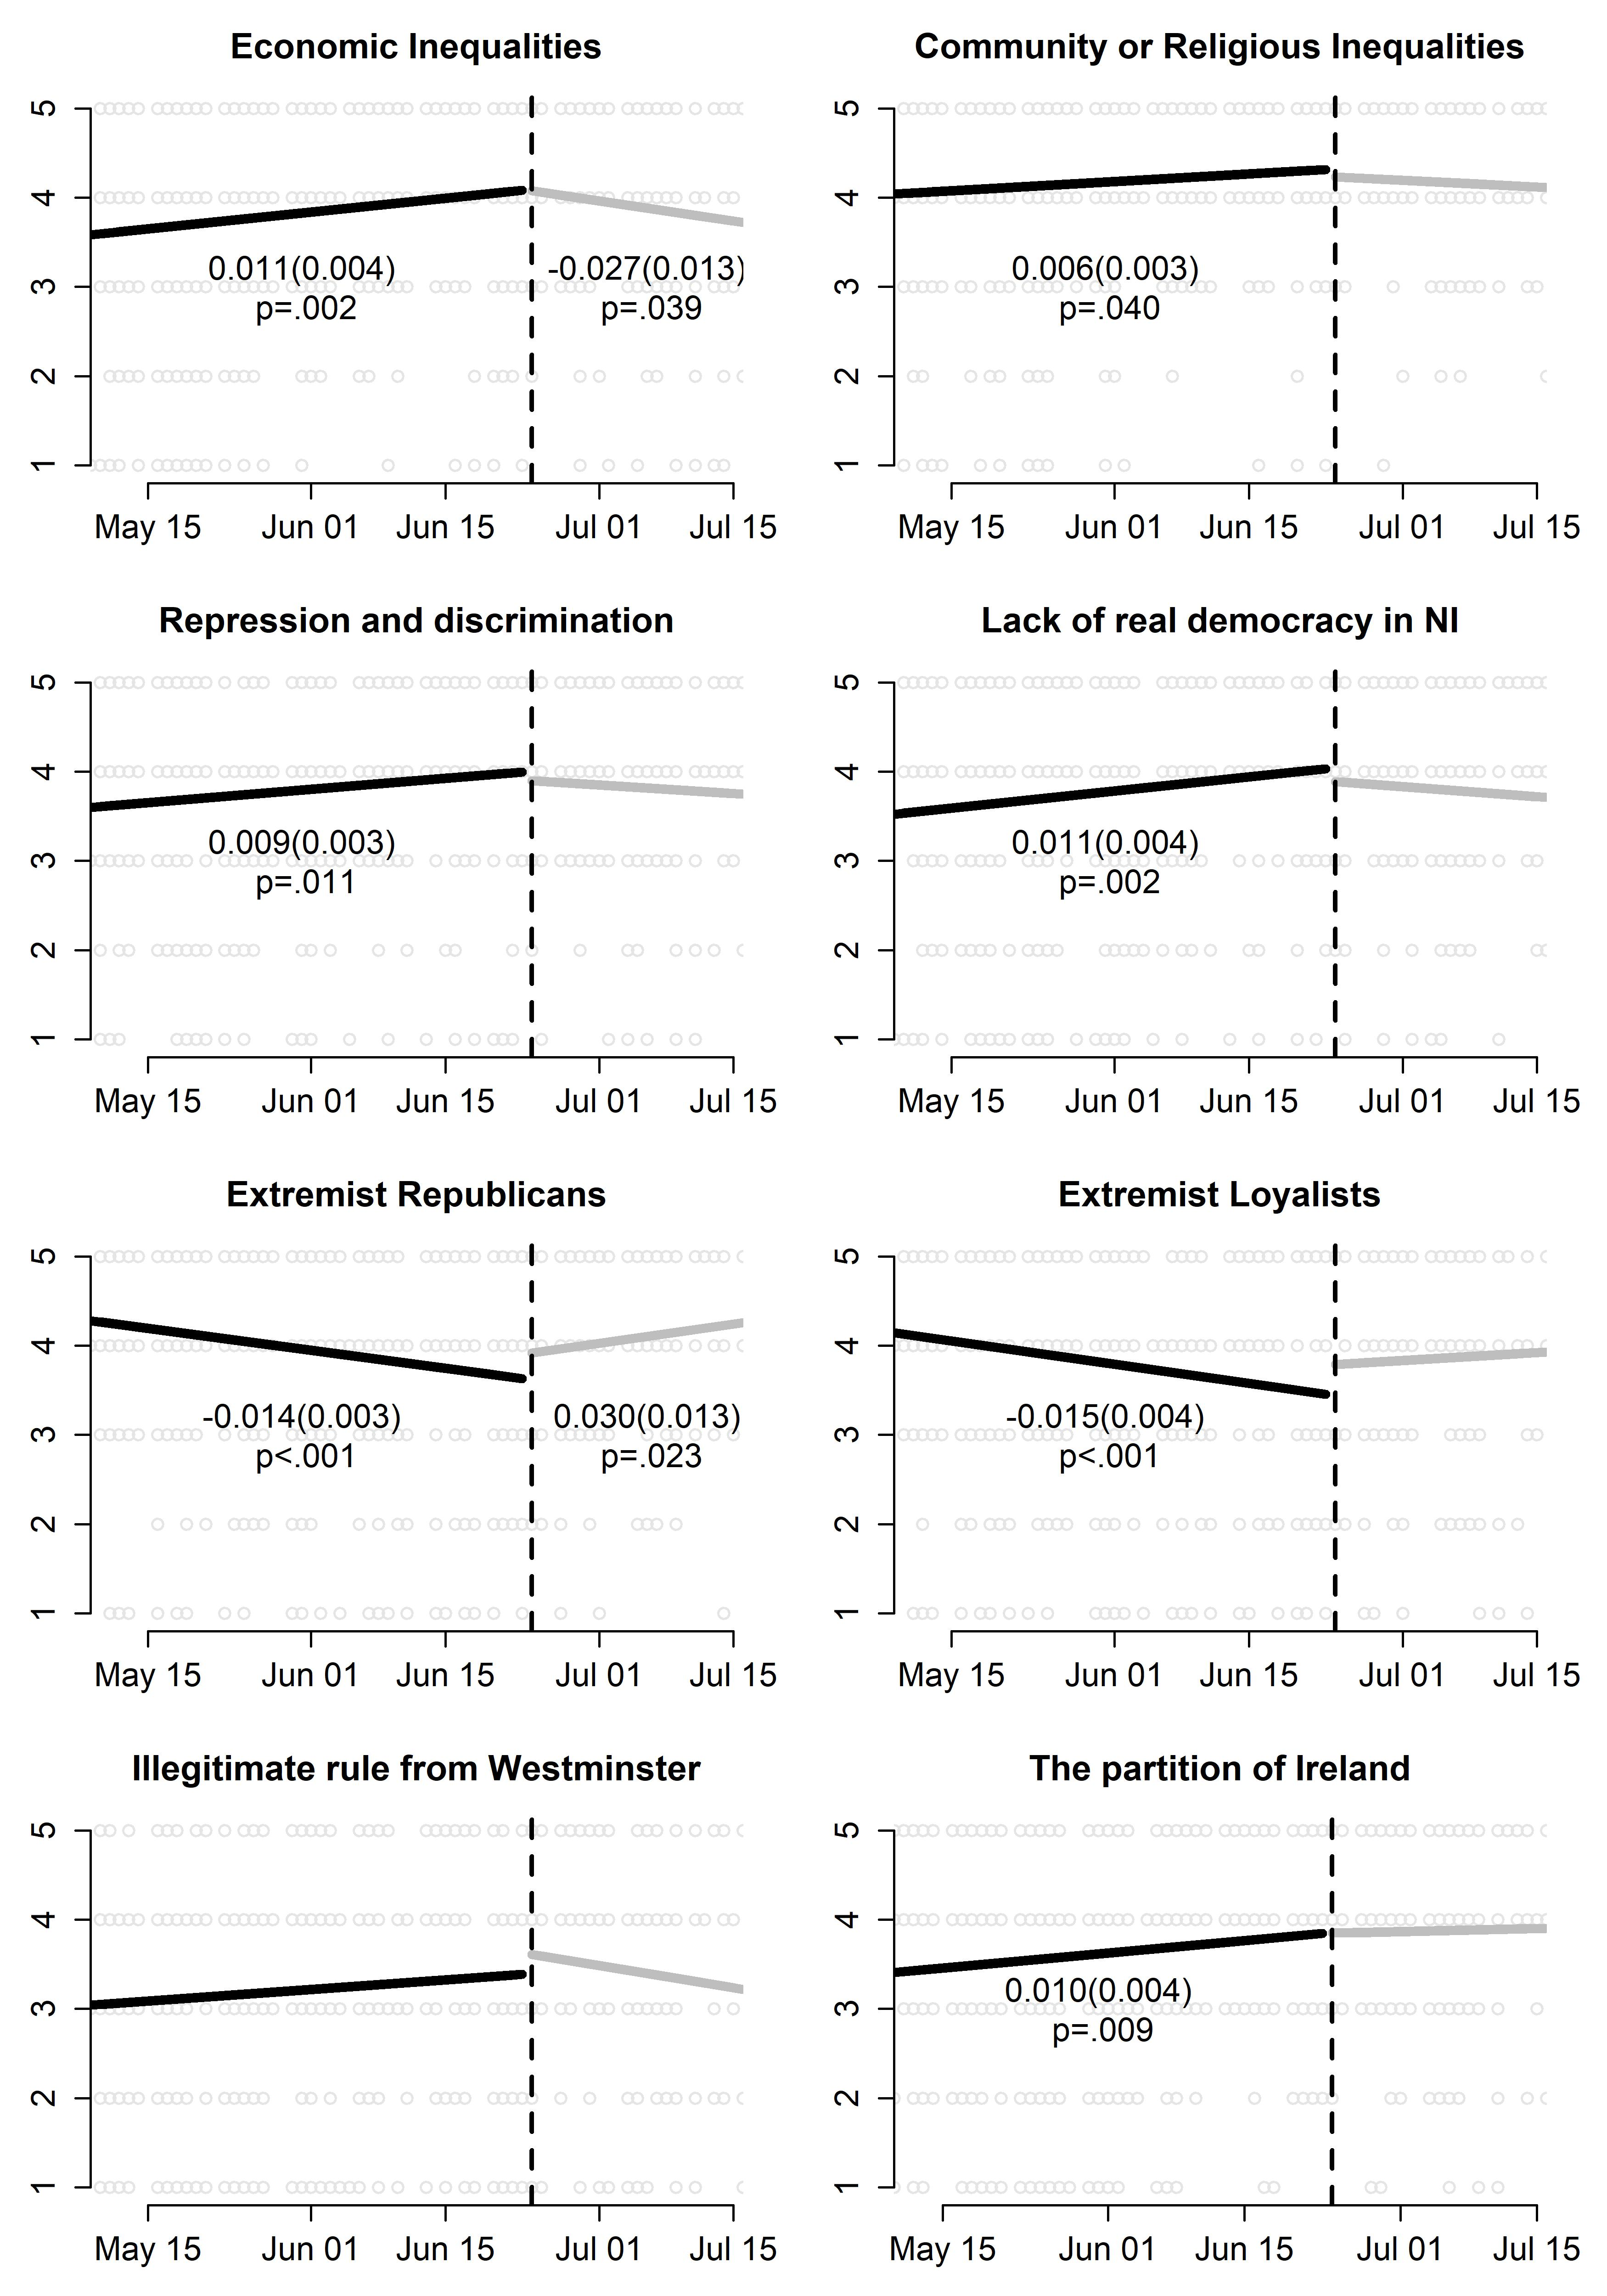
\includegraphics[width=1\textwidth]{Fig4.jpeg}
	\caption{Change in perceptions of conflict causes over time (replicated)}
	\label{fig:meva_figura_4}
\end{figure}
	
	Figure 5 illustrates the gradual evolution of constitutional preferences throughout the Brexit campaign, highlighting that while the shifts were significant, they were ultimately limited in duration as attitudes returned to baseline levels shortly after.\\
	
\begin{lstlisting}[language=R]	
	
	# 1. LAYOUT: Side-by-side comparison (2 panels)
	jpeg("Fig5.jpeg", width = 9, height = 4, units = 'in', res = 500)
	par(mfrow=c(1,2), mar=c(2,2,2,2))
	
	# 2. CORE PLOTTING LOGIC: Unification & Remain
	# Scatter plot of binary outcomes (0/1) against date
	plot(Brexit$date, Brexit$unification, pch=1, col="grey90", 
	frame.plot = FALSE, ylim=c(-0.09, 1.1), main = "Unify with Ireland")
	
	# 3. PREDICTED TREND LINES (RD model)
	# Trend BEFORE (referendum == 0) - Solid Black
	with(subset(Brexit, referendum==0), 
	lines(date, unification.rdd.pred, col="black", lwd=4))
	
	# Trend AFTER (referendum == 1) - Solid Grey
	with(subset(Brexit, referendum==1), 
	lines(date, unification.rdd.pred, col="gray", lwd=4))
	
	# 4. CUTOFF & STATS
	abline(v=as.Date("2016-06-24"), lty=2, lwd=2) # Referendum Threshold
	text(as.Date("2016-05-31"), 0.5, "0.003(0.001)\n p=.018") # Statistical overlay
	
	dev.off()
	
\end{lstlisting}
	
\begin{figure}[h]
	\centering
	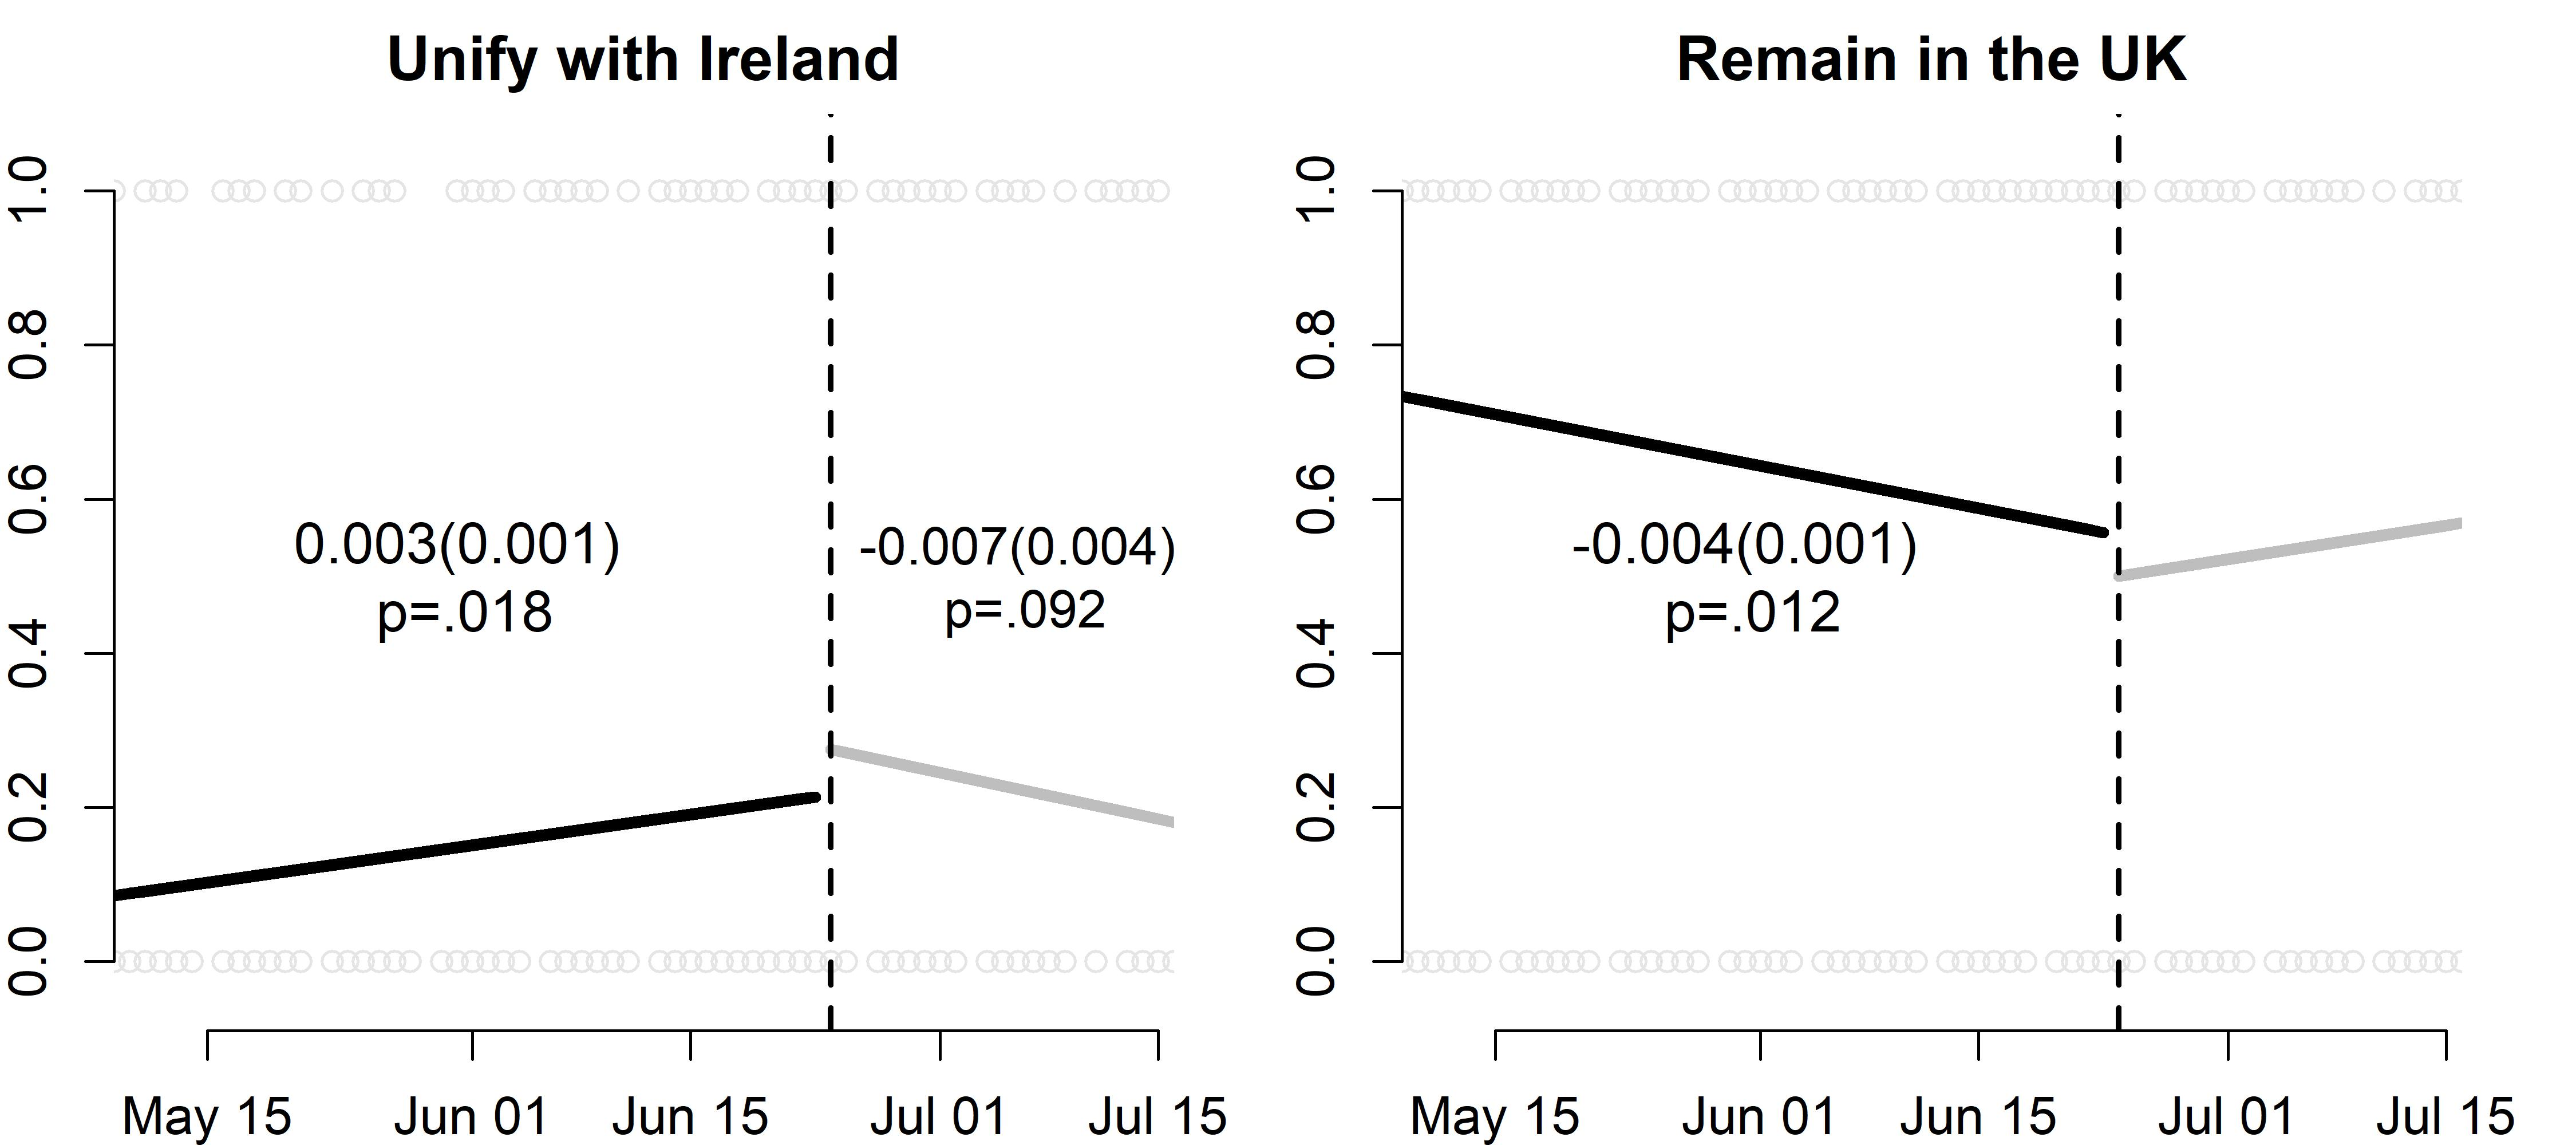
\includegraphics[width=1\textwidth]{Fig5.jpeg}
	\caption{Change in preferences for the future over time (replicated)}
	\label{fig:meva_figura_5}
\end{figure}

	\section{My Contribution: The Differential Effect of the Brexit Referendum on Preferences for Irish Reunification by Age, Exposure to the Troubles, and Gender}
	
	I extend \textcite{godefroidt2023past} by estimating three models in which \texttt{unification} (yes = 1, no = 0) is the dependent variable. Each model includes an interaction term: \texttt{referendum * cohort}, \texttt{referendum * exposure}, and \texttt{referendum * male}. In doing so, I assess whether the change in preferences for Irish reunification following the Brexit referendum varies across age cohorts, between individuals exposed and not exposed to \textit{the Troubles}, and across gender.\\

The code corresponding to this extension begins at line 826 of the R script. Nevertheless, I reproduce below the code for the GLM models.\\

\subsection{1st Interaction Model: Cohort}

The first step consists in constructing a variable labelled \texttt{cohort}. Given that the survey was conducted in 2016 and that \textit{the Troubles} had ended 18 years earlier, I define three age groups. The first group (18–25) includes individuals who were infants or young children at the end of the conflict. The second group (26–45) comprises individuals who were young or in early adulthood. The third group (over 45) includes those who were at least 28 years old when \textit{the Troubles} ended. This final group is used as the reference category in the analysis.\\

\begin{lstlisting}[language=R]	
Brexit.ext$cohort <- cut(Brexit.ext$age, 
breaks = c(18, 25, 45, Inf), 
labels = c("18-25", "26-45", "Over 45"),
include.lowest = TRUE)

Brexit.ext$cohort <- relevel(Brexit.ext$cohort, ref = "Over 45")
\end{lstlisting}

As in the original study, I then recalculated the weights for this specification:\\

\begin{lstlisting}[language=R]	
W.ext <- weightit(referendum ~ age + employment_1 + exposure + cohort, 
data = Brexit.ext, 
estimand = "ATT", 
method = "ebal")
\end{lstlisting}

Finally, I estimated the model:\\

\begin{lstlisting}[language=R]	
ext_model_cohorts_uni <- glm(unification ~ referendum * cohort + education + employment_1 + exposure, 
data = Brexit.ext, 
family = binomial(link = "logit"),
weights = W.ext$weights)
\end{lstlisting}

The results presented in Figure 6 indicate that the referendum did not produce a differential effect on preferences for reunification across age cohorts. Rather, the Brexit referendum appears to have acted as a broad systemic shock, increasing the probability of support for Irish reunification across all age groups. While the youngest cohort (18–25) displays a higher baseline level of support, the over-45 cohort exhibits a more precise and substantial increase, approximately doubling its initial probability.\\

However, the non-significant interaction term is consistent with the visual evidence, as reflected in the relatively parallel upward shifts observed across cohorts. However, the wider confidence intervals for the youngest group suggest greater variability in their response to the referendum.\\

\begin{figure}[h]
	\centering
	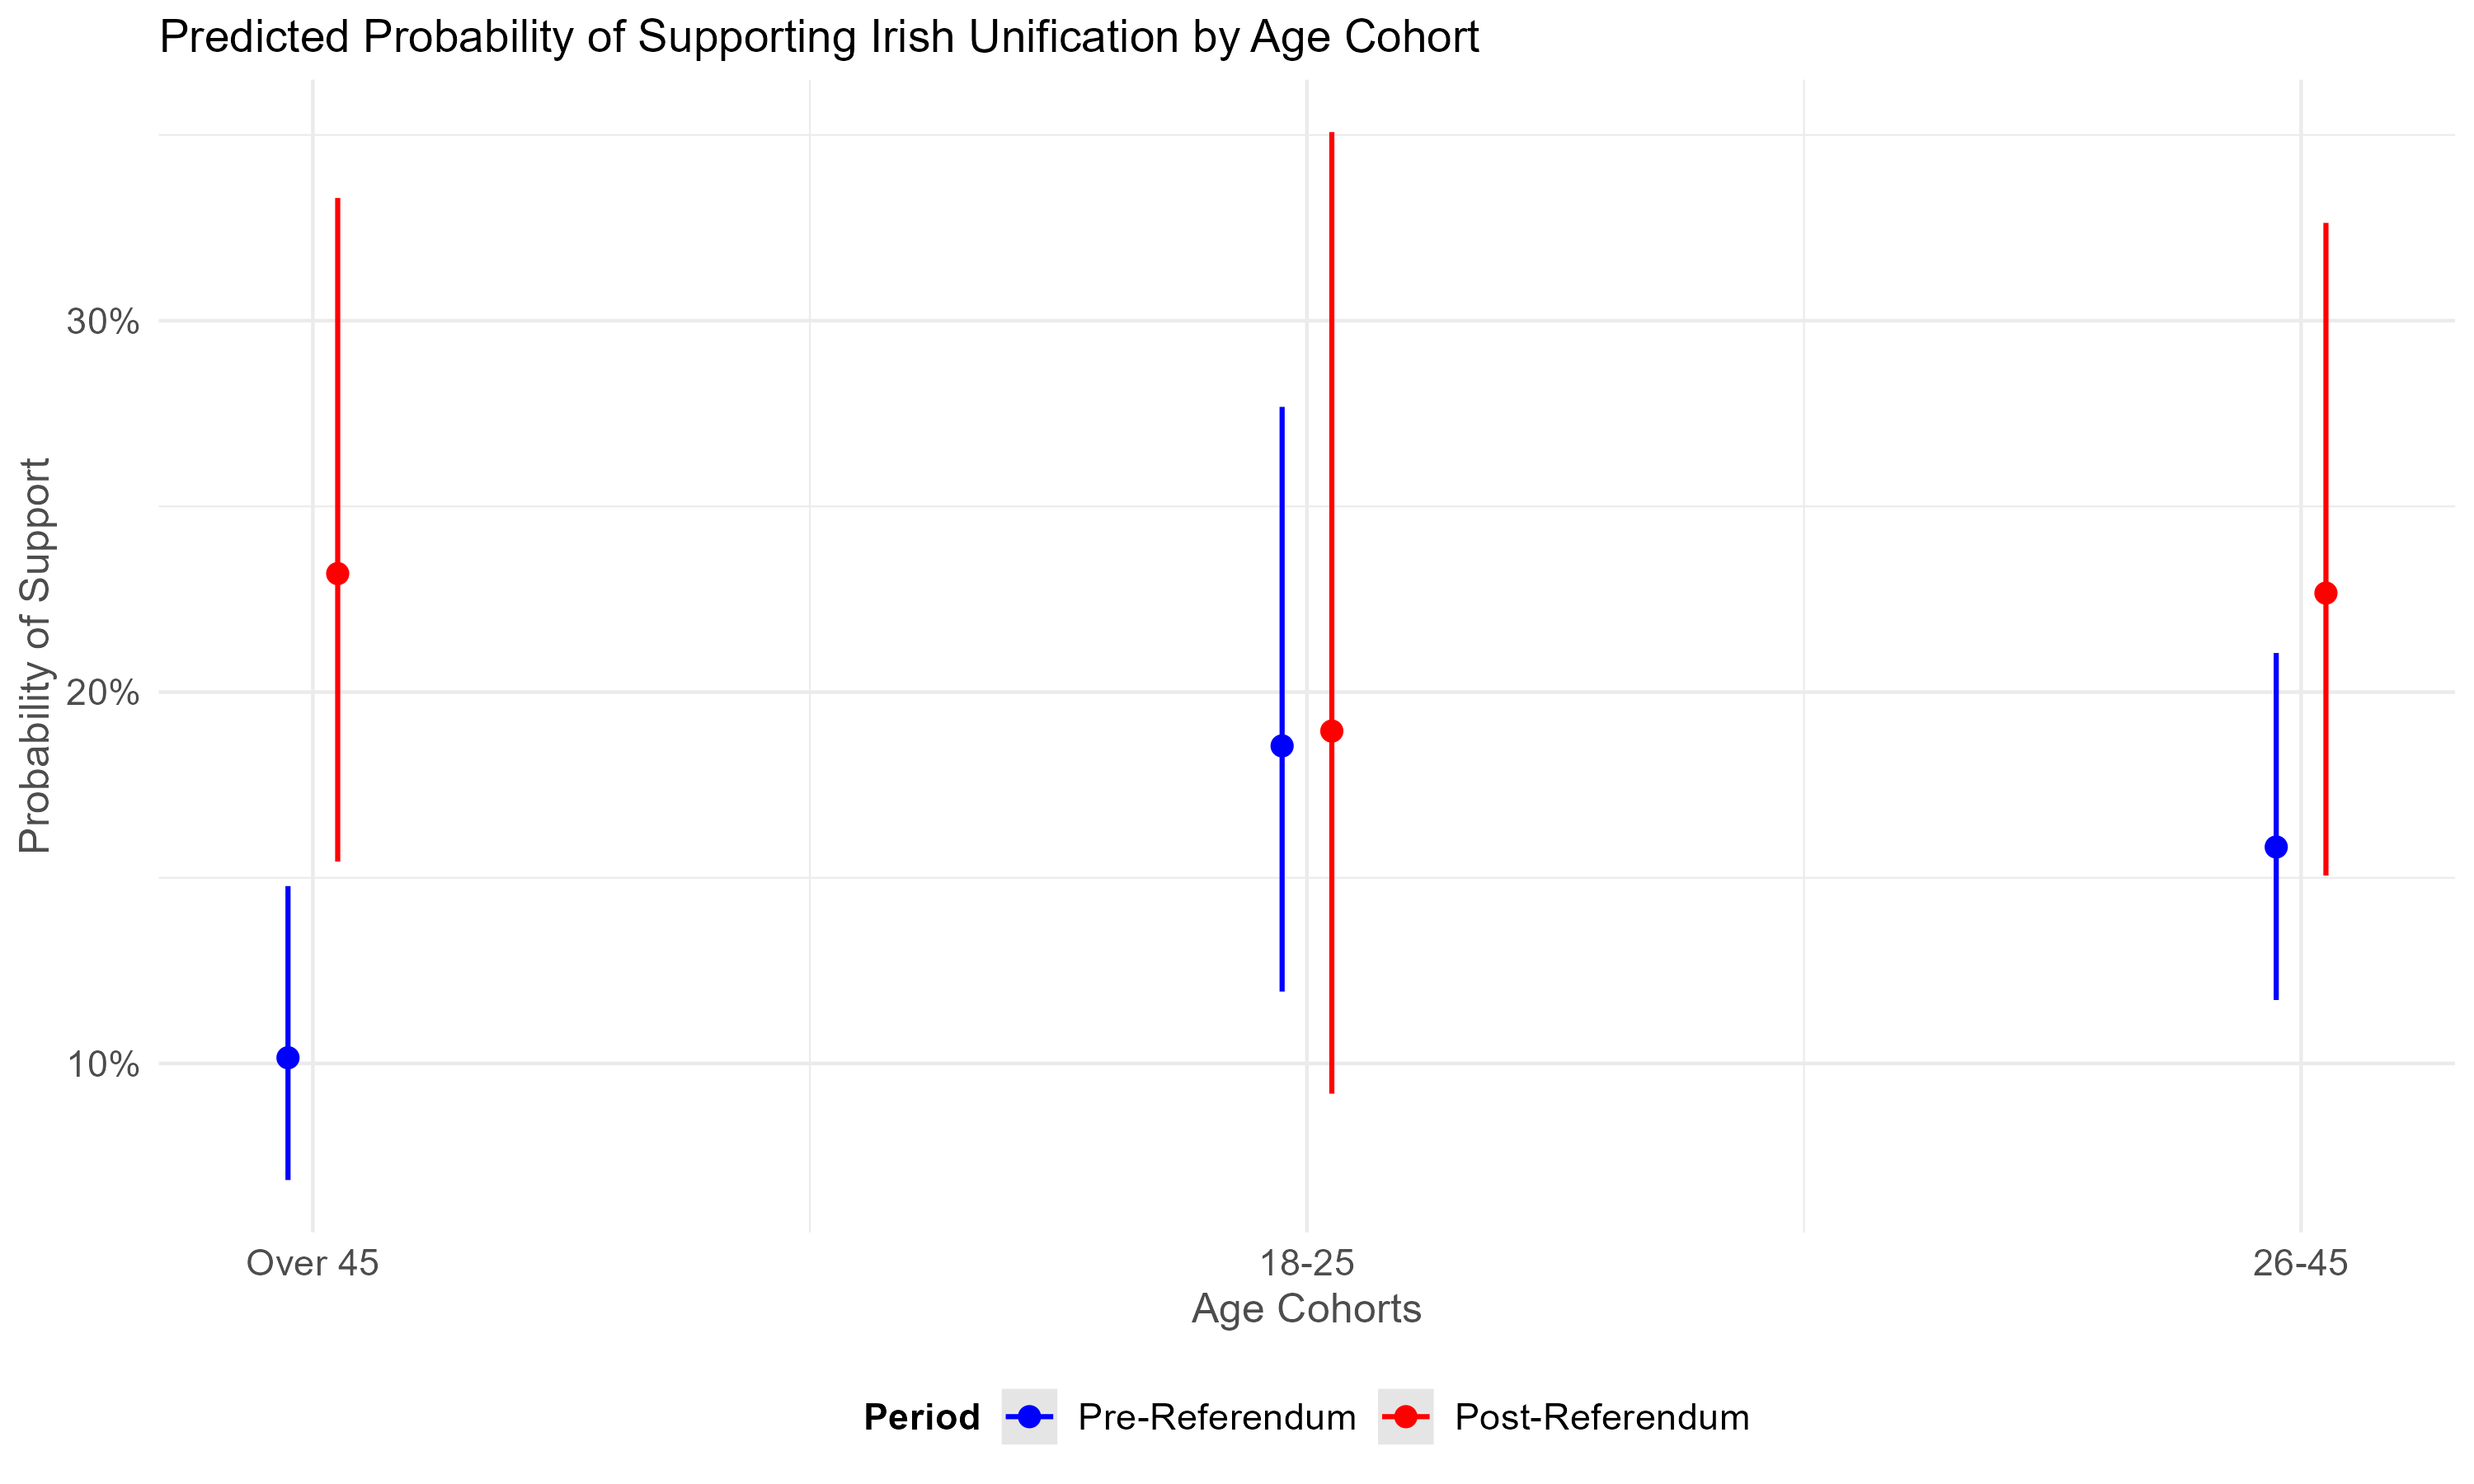
\includegraphics[width=1\textwidth]{plot_ext1.png}
	\caption{Change in preferences for Irish reunification by cohort}
	\label{fig:meva_figura_6}
\end{figure}

\subsection{2nd Interaction Model: Exposure}

An important variable in the survey is \texttt{exposure} (yes = 1, no = 0), indicating whether the respondent was a victim of \textit{the Troubles}. The purpose of this model is to assess whether the effect of the Brexit referendum on preferences for reunification with the Republic of Ireland differed between individuals who had been victims of the conflict and those who had not.\\

\begin{lstlisting}[language=R]	
ext_model_exposure_uni <- glm(unification ~ referendum * exposure + cohort + education + employment_1, 
data = Brexit.ext, 
family = binomial(link = "logit"),
weights = W.ext$weights)
\end{lstlisting}

The results shown in Figure 7 indicate that victims of \textit{the Troubles} were already slightly more inclined to support reunification, and that the referendum--as \textcite{godefroidt2023past} had demonstrated--led to a general increase in support. Importantly, the increase among victims was substantially larger than among non-victims. This finding suggests that the outcome of the referendum had a stronger effect on those who had experienced the trauma of ethno-nationalist violence firsthand.

\begin{figure}[h]
	\centering
	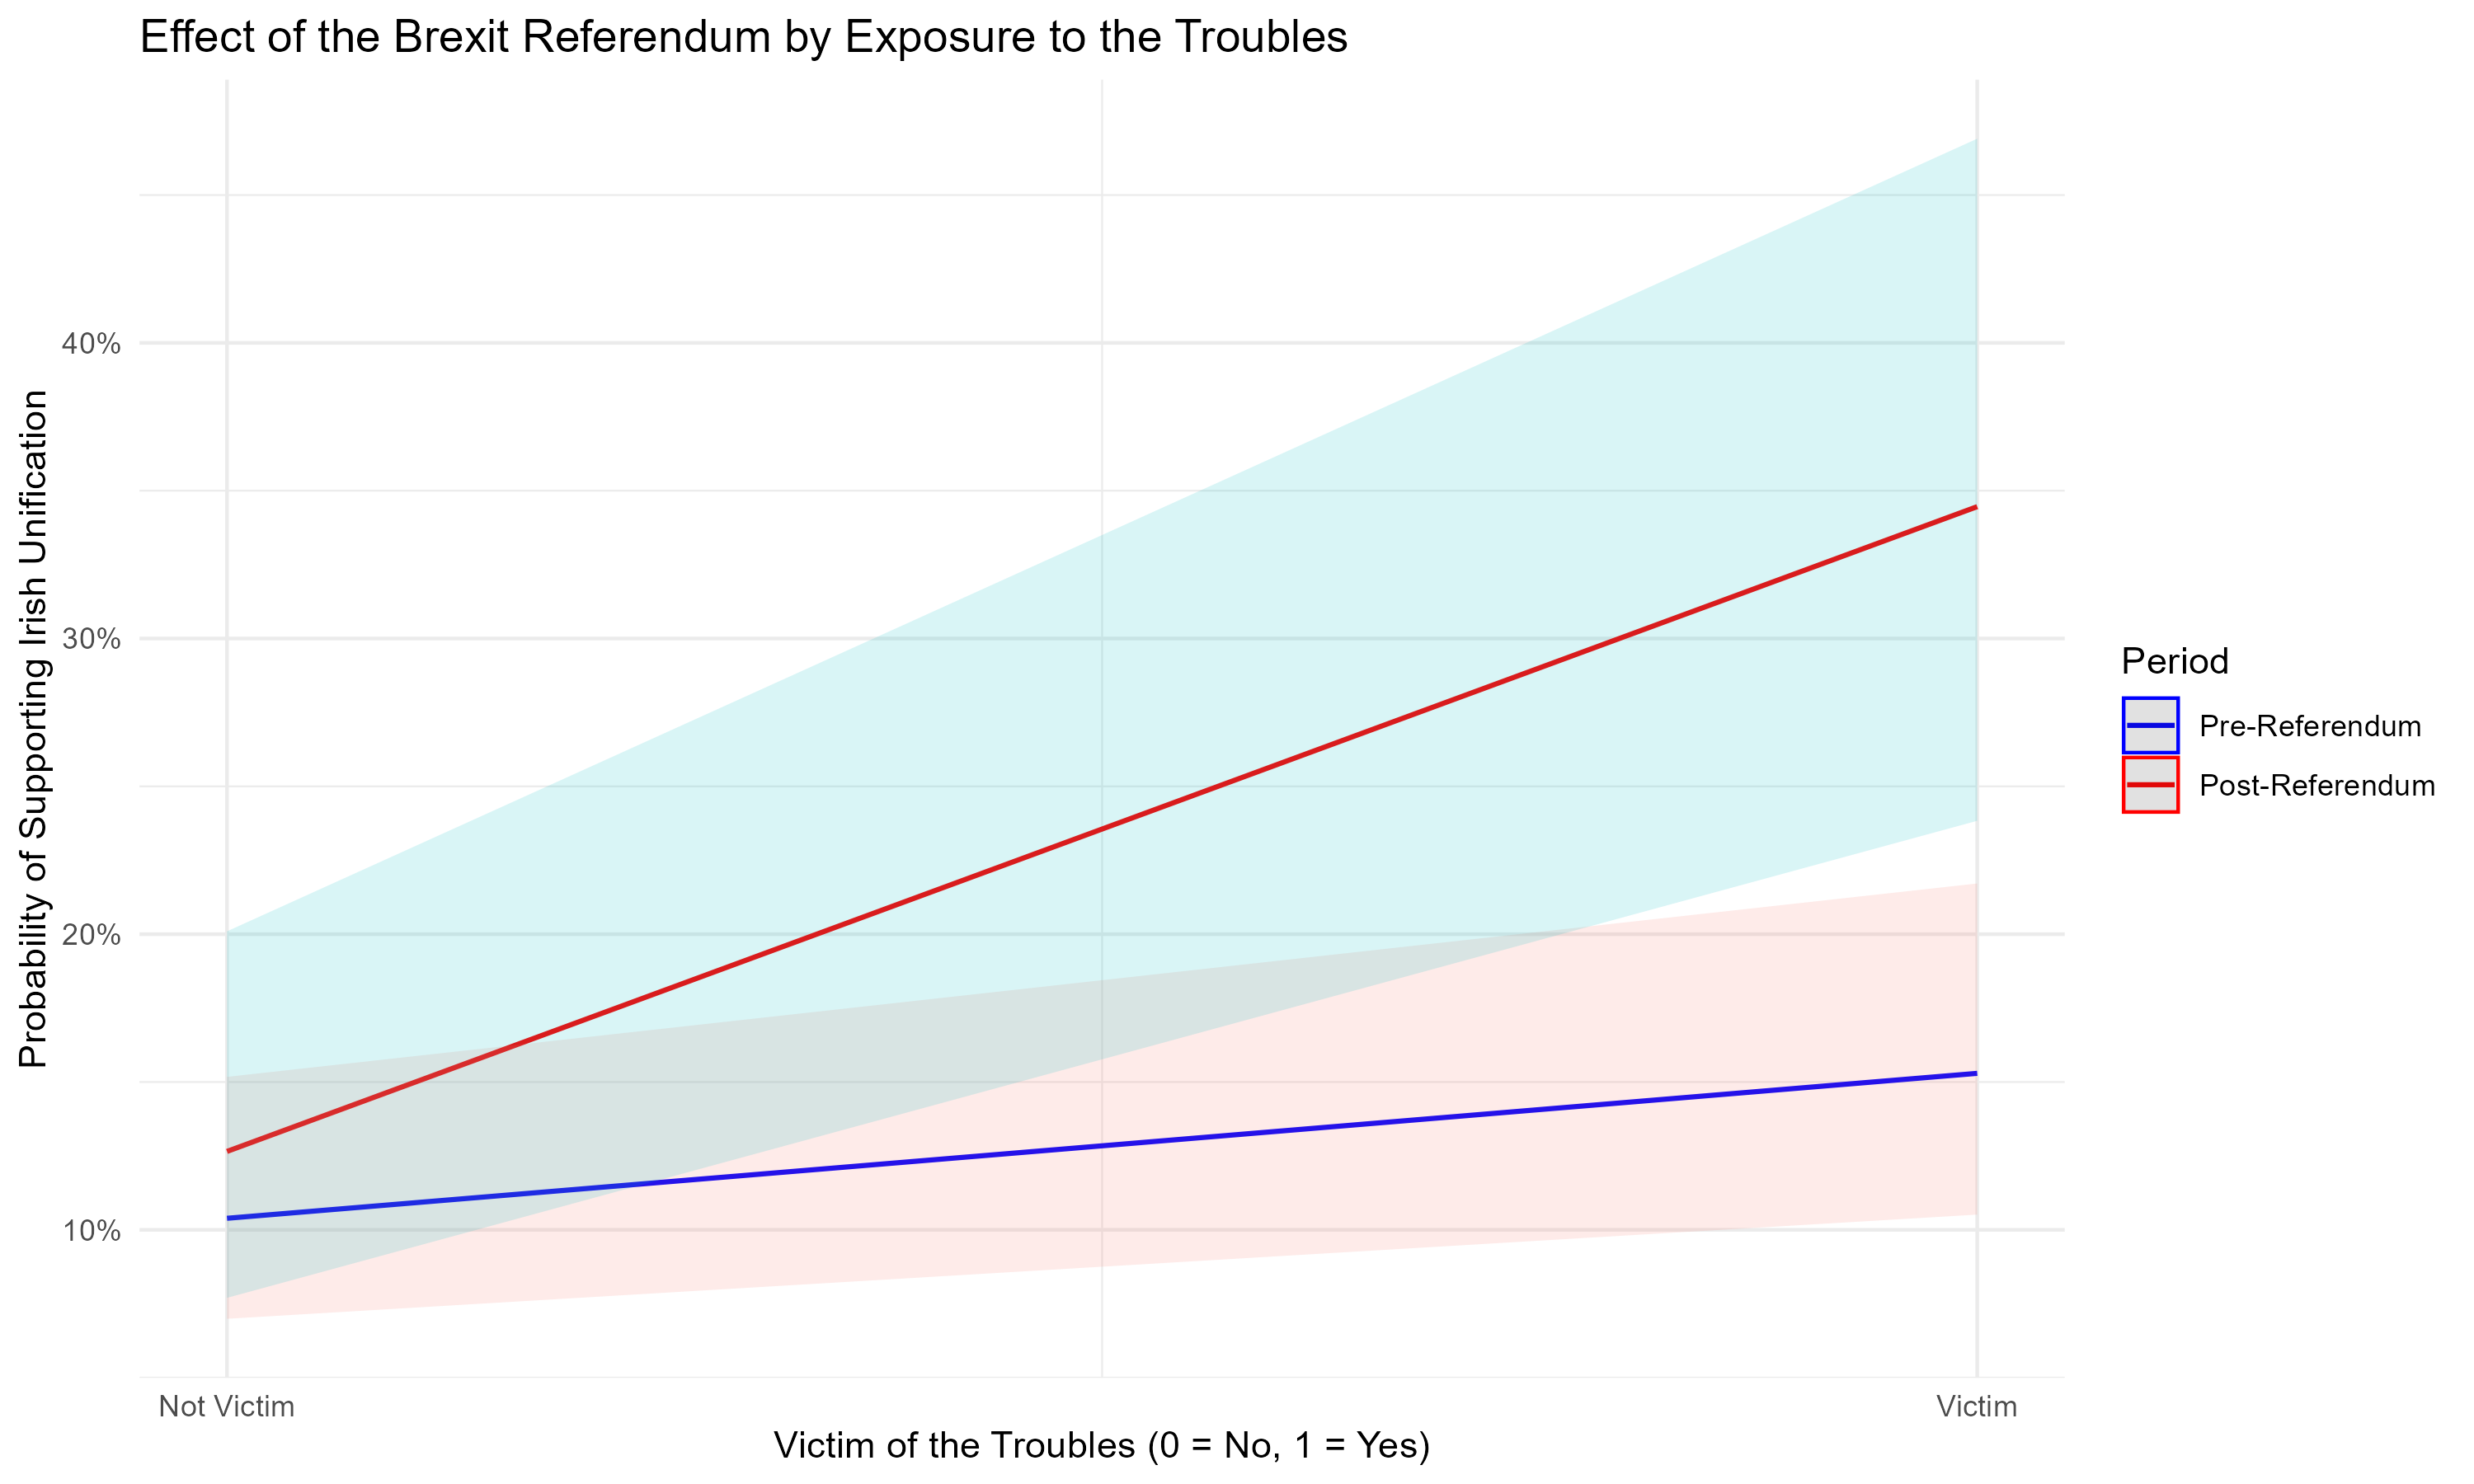
\includegraphics[width=1\textwidth]{plot_ext2.png}
	\caption{Change in preferences for Irish reunification by firsthand exposure to the Troubles}
	\label{fig:meva_figura_7}
\end{figure}

\subsection{3rd Interaction Model: Gender}

The replication dataset also includes a variable \texttt{male} (yes = 1, no = 0, indicating women). By including an interaction term \texttt{referendum * male}, while controlling for other variables such as \texttt{age} and \texttt{exposure}, it is possible to assess whether the effect of the referendum differed between men and women.\\

\begin{lstlisting}[language=R]	
ext_model_exposure_sex <- glm(unification ~ referendum * male + age + exposure + education + employment_1, 
data = Brexit.ext.sex, 
family = binomial(link = "logit"),
weights = W.ext_sex$weights)
\end{lstlisting}

Interestingly, the results in Figure 8 indicate that the effect of the Brexit referendum was considerably stronger for men than for women. While further research would be needed to confirm the underlying mechanisms, one plausible interpretation is that support for Irish nationalism may be somewhat associated with masculinity, or, as has often been suggested, women tend to be more risk-averse than men and therefore less likely to endorse radical changes, such as altering the constitutional status of their country. 

\begin{figure}[h]
	\centering
	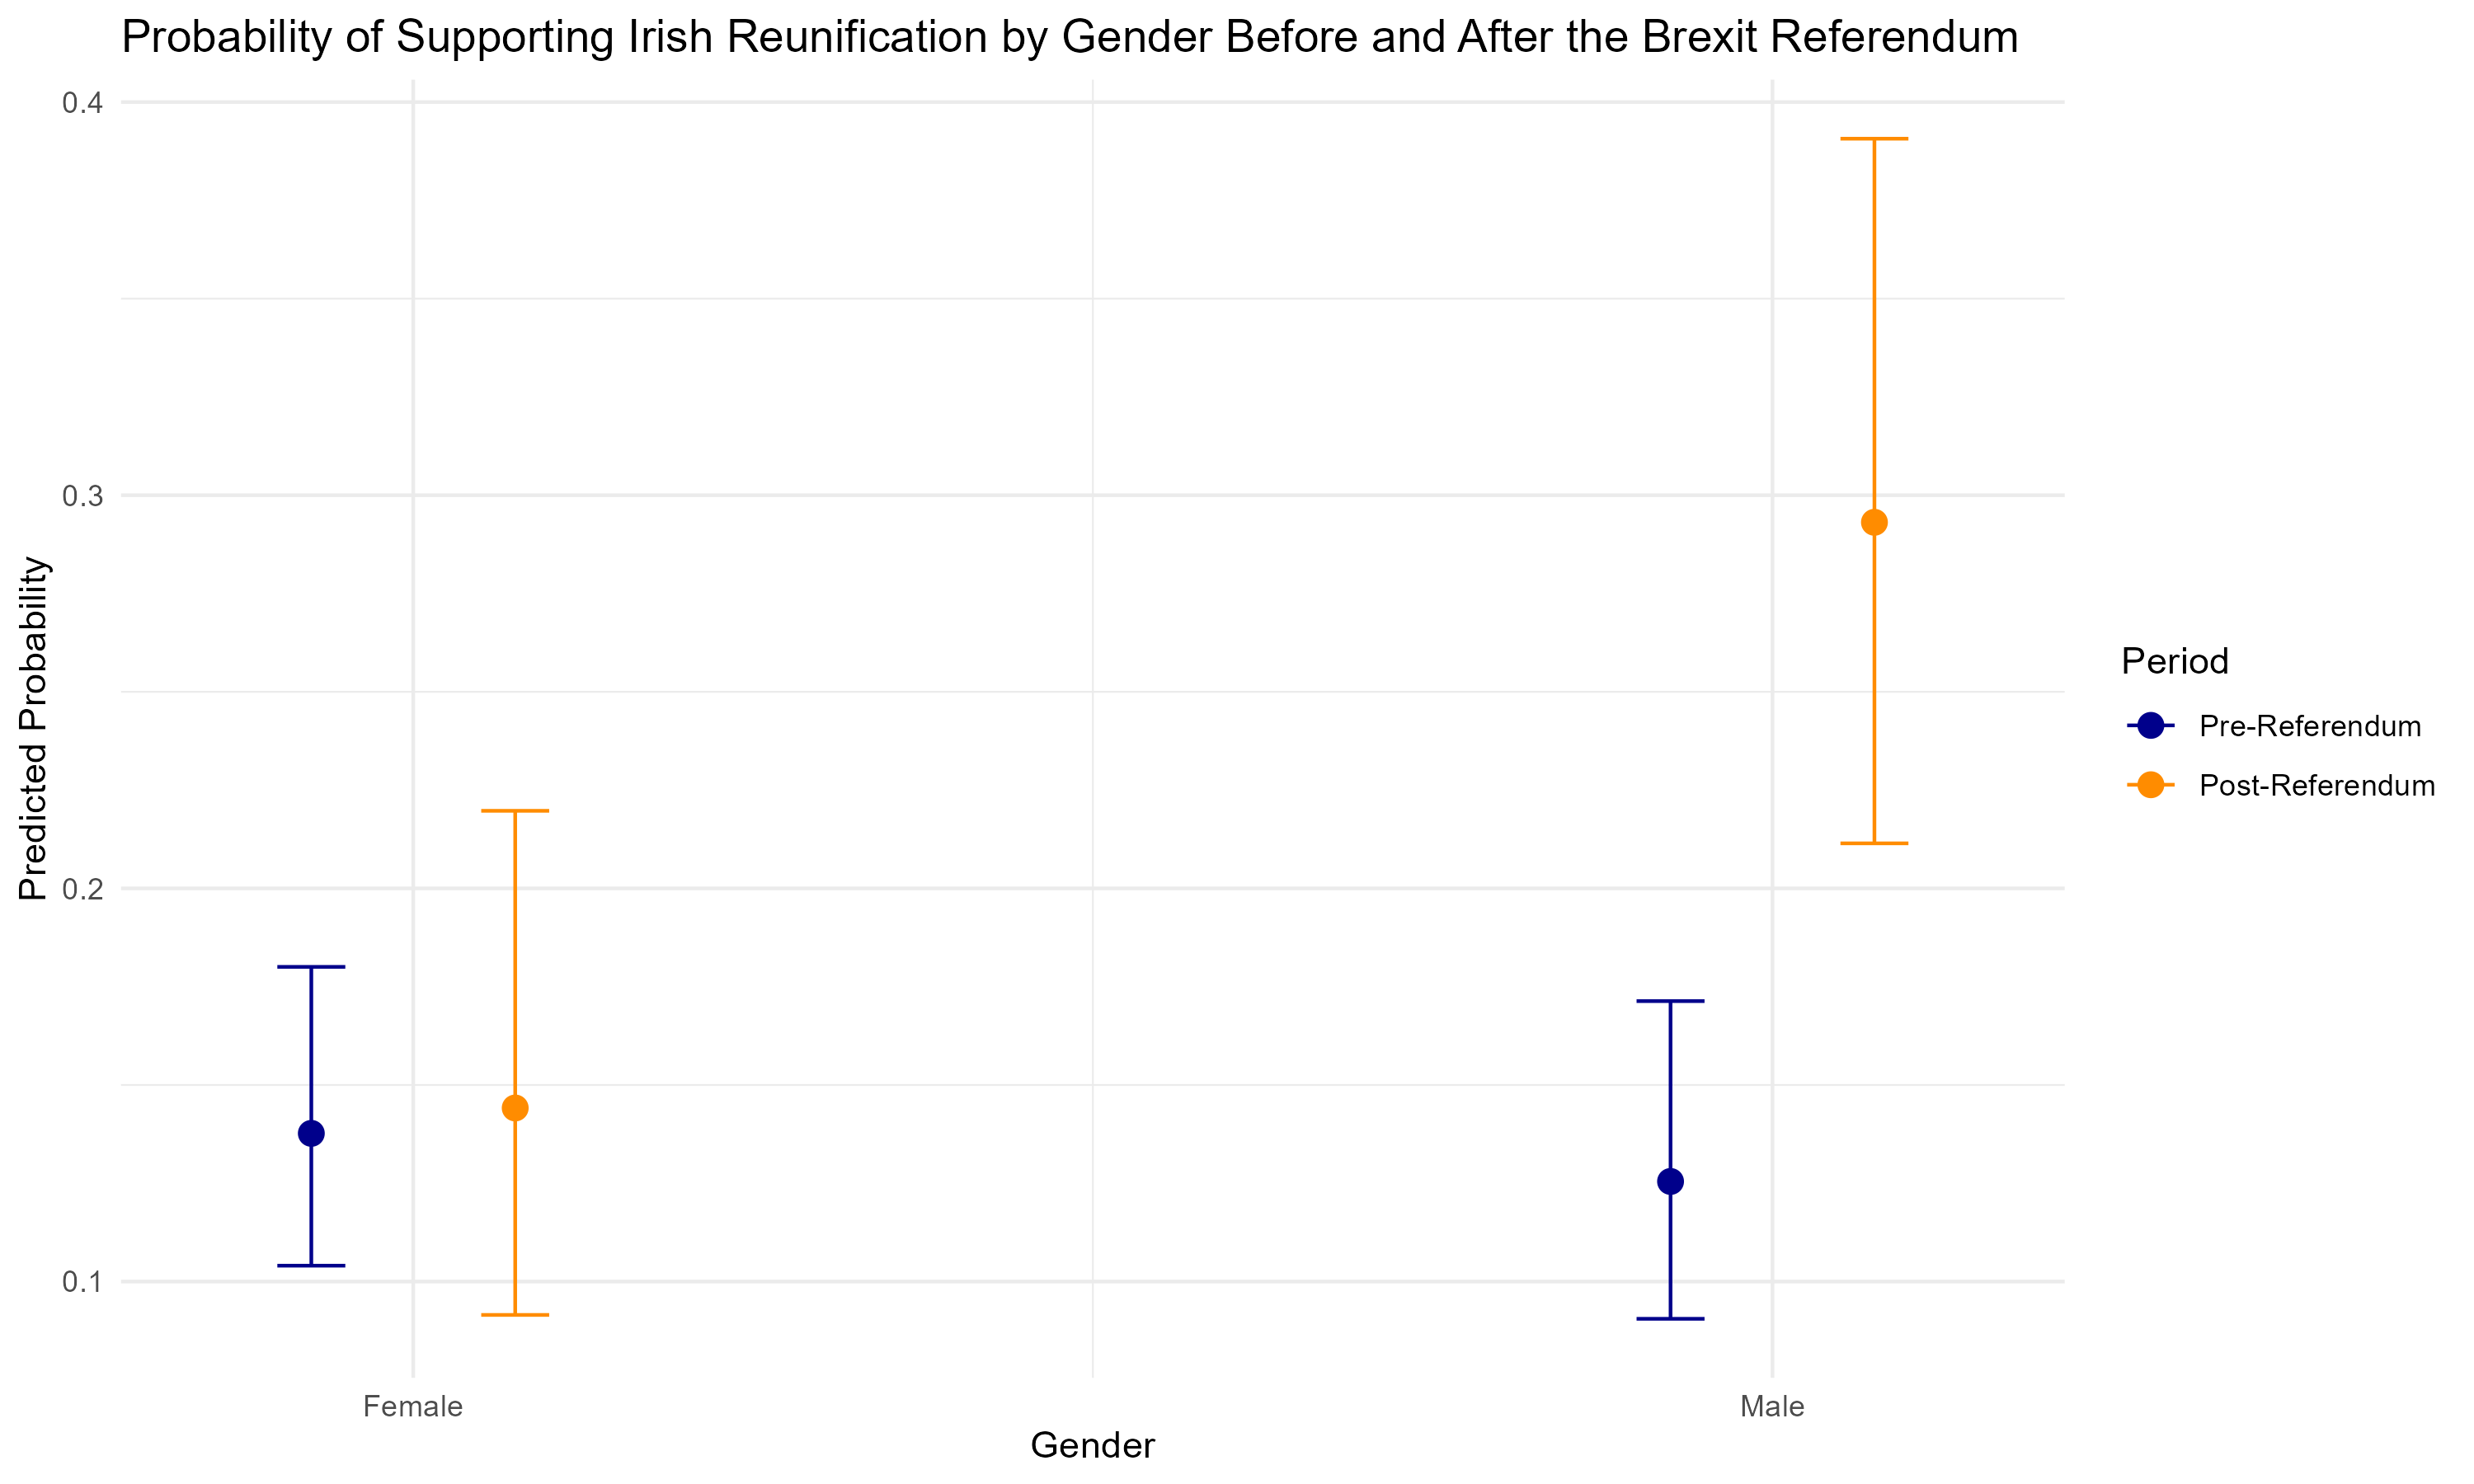
\includegraphics[width=1\textwidth]{plot_ext3.png}
	\caption{Change in preferences for Irish reunification by gender}
	\label{fig:meva_figura_8}
\end{figure}

	\section{Bibliography}
\printbibliography
\end{document}
